\chapter{PicnicAuth}

\section{Architektura projektu}
Projekt składa się z trzech komponentów: serwera w architekturze REST (Representational state transfer) API, 
informacyjnej strony internetowej oraz bibliotek klienckich. Komponenty te są od siebie niezależne, dzięki czemu 
łatwa jest rozbudowa projektu, jak również wersjonowanie każdego z nich.

\subsection{REST API}
Pierwszym z nich jest serwer implementujący logikę aplikacji. 
Jest on stworzony w technologii \textit{ASP.NET Web API 2} w języku programowania \textit{C\#}. \\
Przy jego tworzeniu zostały zachowane zasady architektury REST, co pozwala na łatwą i sprawną integracją
platform klienckim, niezależnie od użytej technologii. \\ \\
Zasoby udostępniane przez REST API to:
\begin{itemize}
	\item \textit{[GET] /api/Companies/Me/AuthUsers} \\
		Zwraca listę użytkowników dla aktualnie zalogowanego podmiotu.
	\item \textit{[POST] /api/AuthUsers} \\
		Tworzy nowego użytkownika i dodaje go do kolekcji użytkowników zalogowanego podmiotu.
		W odpowiedzi zwracany jest sekret stworzonego użytkownika, jak również link 
		do kodu QR kompatybilnego z aplikacjami mobilnymi.
	\item \textit{[PATCH] /api/AuthUsers/{userId}/secret} \\
		Generuje nowy sekret dla użytkownika o podanym \textit{userdId}.
	\item \textit{[GET] /api/Companies/Me} \\ 
		Zwraca dane zalogowanego podmiotu, takie jak login, adres poczty elektronicznej oraz unikalny identyfikator.
	\item \textit{[POST] /api/Companies} \\
		Tworzy nowe konto podmiotu. 
	\item \textit{[GET] /api/AuthUsers/{userId}/hotp} \\
		Zwraca hasło jednorazowe typu \textit{HOTP} dla użytkownika o podanym \textit{userId}.
	\item \textit{[GET] /api/AuthUsers/{userId}/totp} \\
		Zwraca hasło jednorazowe typu \textit{TOTP} dla użytkownika o podanym \textit{userId}.
	\item \textit{[GET] /api/AuthUsers/{userId}/hotp/{hotp}} \\
		Zwraca wynik weryfikacji podanego hasła jednorazowego typu \textit{HOTP}
	\item \textit{[GET] /api/AuthUsers/{userId}/totp/{totp}} \\
		Zwraca wynik weryfikacji podanego hasła jednorazowego typu \textit{TOTP}
	\item \textit{[POST] /api/tokens}
		Zwraca klucz API, który służy do uwierzytelnienia podmiotu. (Równoznaczne z logowaniem,
		zgodnym ze standardem \textit{OAuth}.)
\end{itemize}
Zasoby na których operuje API są w formacie JSON (JavaScript Object Notation), zarówno przy metodach, które
przyjmują dane, jak i tych, które zwracają dane. \\
Za pomocą pakietu \textit{Swashbuckle} skonfigurowana została automatyczna generacja dokumentacji API
na podstawie publicznie wystawionych kontrolerów. 
Oprócz podstawowych informacji o metodach znajdujących się w kontrolerach, takich jak nazwy czy typy parametrów, 
w~dokumentacji umieszczane są także komentarze, którymi opisana jest dana metoda. Oprócz funkcji informacyjnej, 
wygenerowana dokumentacja pozwala na wygodne testy każdej z metod. 
Końcowy efekt wygenerowanej dokumentacji przedstawiony jest na Rysunku \ref{swagger}. \\
Aplikacja przeznaczona jest do działania na serwerze \textit{IIS (Internet Information Service)} w~wersji~7.
\begin{figure}[t]
    \centering
	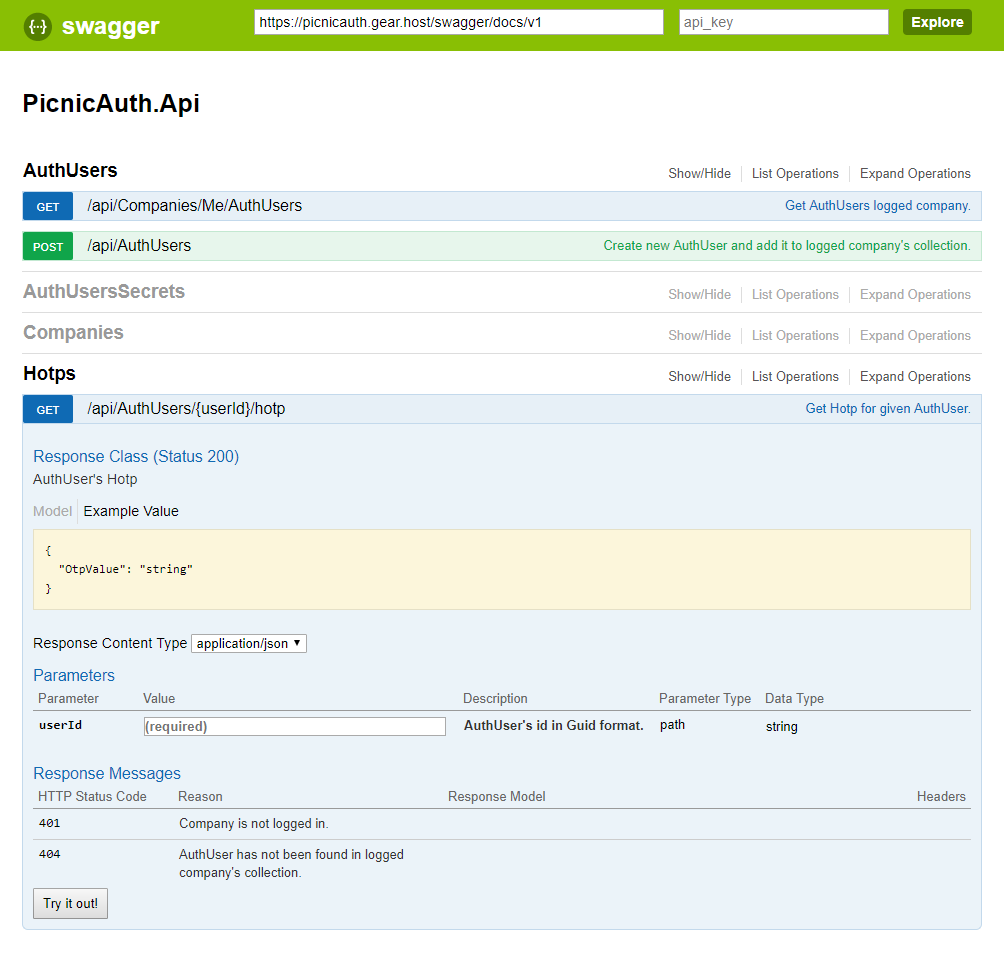
\includegraphics[width=\textwidth]{content/images/swagger}
    \caption{Interaktywna dokumentacja API.}
    \label{swagger}
\end{figure}

\subsection{Frontend}
Strona internetowa projektu (Rysunek \ref{front-home}) stworzona została w technologii \textit{Angular} w wersji~5 w konwencji 
\textit{Single Page Application}. Znajduje się na niej instrukcja użycie projektu jak również informacje
o aktualnej liczbie dostępnych bibliotek. Zawiera ona także przydatne odnośniki do repozytoriów, w których
znajduje się kod źródłowy oraz do strony na której znajduje się dokumentacja API. \\
Dodatkowymi funkcjonalnościami jakie oferuje strona jest stworzenie nowego konta dla podmiotu 
(przedstawione na Rysunku \ref{front-create}), jak również uzyskanie klucza API, 
umożliwiającego użycie bibliotek klienckich.
\begin{figure}[t]
    \centering
	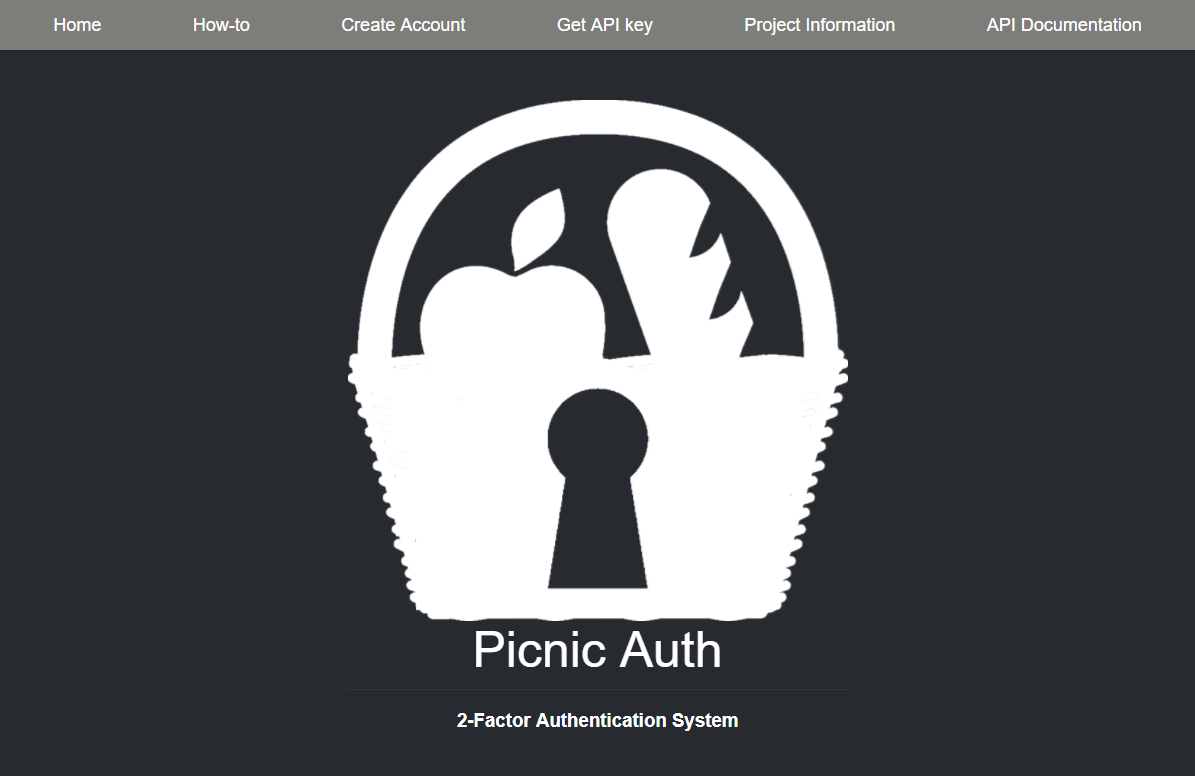
\includegraphics[width=\textwidth]{content/images/front-home}
    \caption{Informacyjna strona internetowa projektu.}
    \label{front-home}
\end{figure}
\begin{figure}[t]
    \centering
	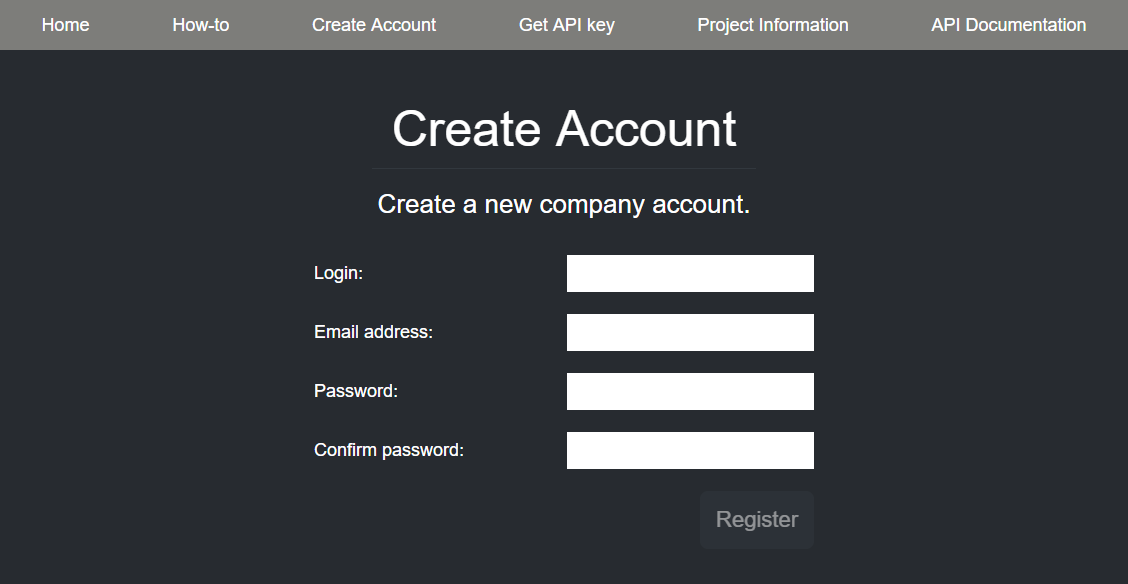
\includegraphics[width=\textwidth]{content/images/front-create}
    \caption{Tworzenie konta podmiotu.}
    \label{front-create}
\end{figure}

\subsection{Biblioteki klienckie}
W celu ułatwienia integracji z serwerem zaimplementowane zostały biblioteki klienckie.
Umożliwiają one w prosty sposób użycie funkcjonalności serwera bez konieczności 
studiowania dokumentacji i pisania kodu odpowiedzialnego za integrację. \\
Przykładowo biblioteka w języku C\# udostępnia klasę \textit{PicnicAuthClient}, posiadająca metody:
\begin{itemize}
	\item Login
	\item GetAuthUsers
	\item AddAuthUser
	\item GenereteNewSecret
	\item GetLoggedCompany
	\item AddCompany
	\item GetHotpForAuthUser
	\item ValidateHotpForAuthUser
	\item GetTotpForAuthUser
	\item ValidateTotpForAuthUser
\end{itemize}
Na chwilę obecną gotowe do użycia są biblioteki w następujących technologiach:
\begin{enumerate}
	\item C\#
	\item Visual Basic
	\item TypeScript
	\item Python 3.6
	\item Python 2.7
	\item Ruby
\end{enumerate}

\section{Dostarczanie sekretu na urządzenie mobilne}
\begin{figure}[t]
    \centering
	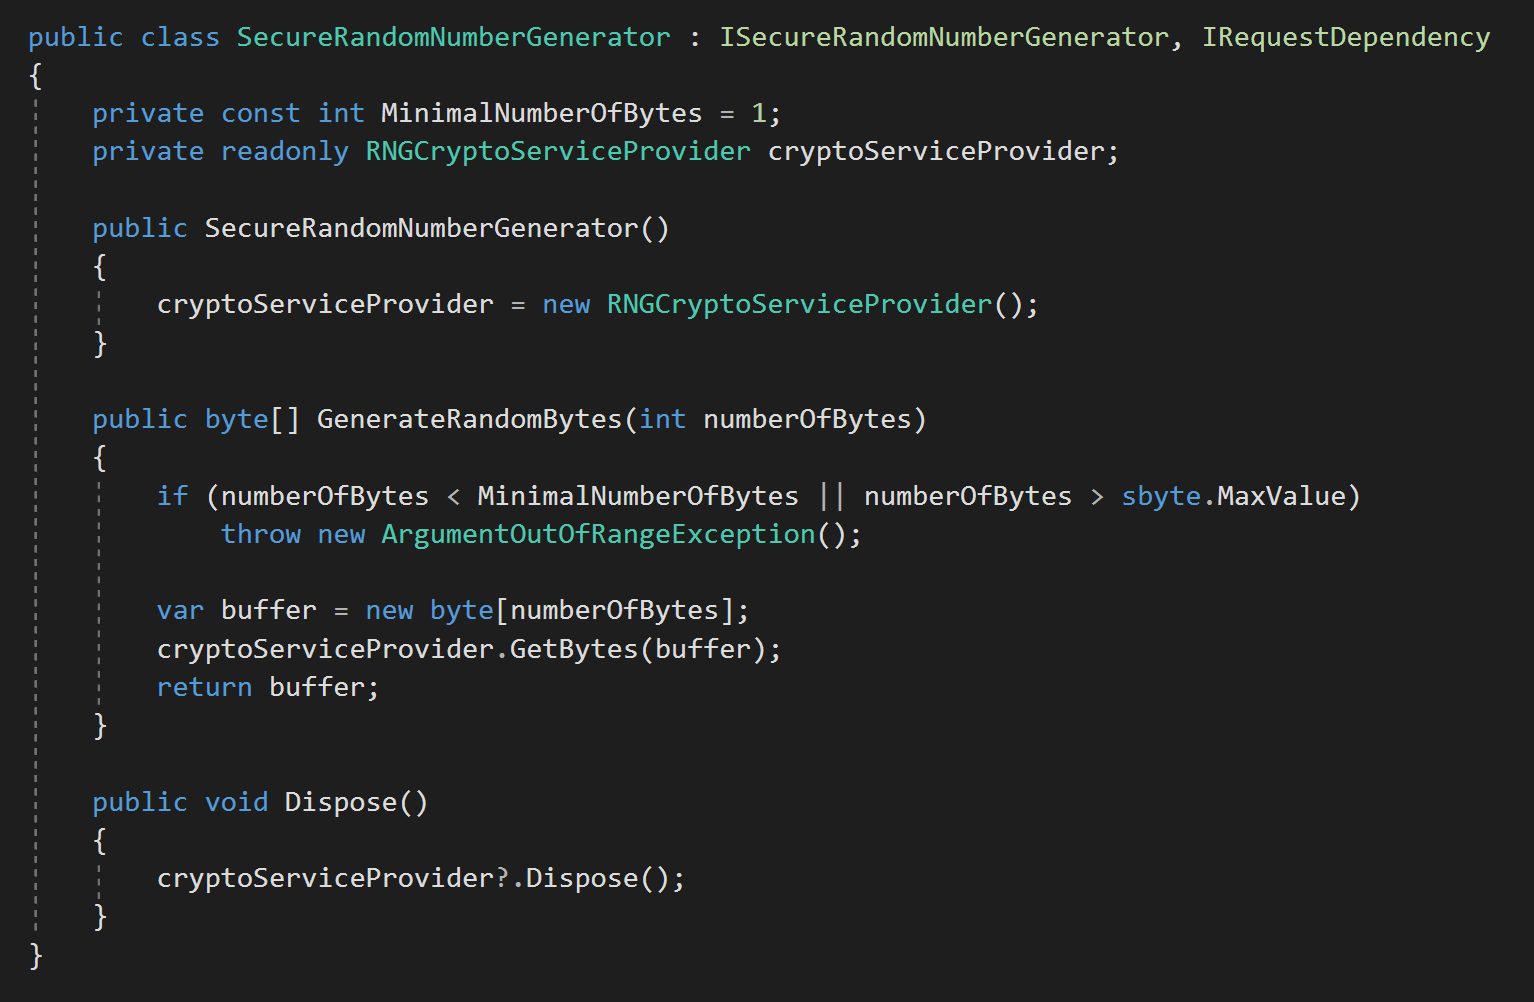
\includegraphics[width=\textwidth]{content/images/code-srng}
    \caption{Klasa zwracająca kryptograficznie bezpiecznie pseudolosowe dane.}
    \label{code-srng}
\end{figure}
\begin{figure}[t]
    \centering
	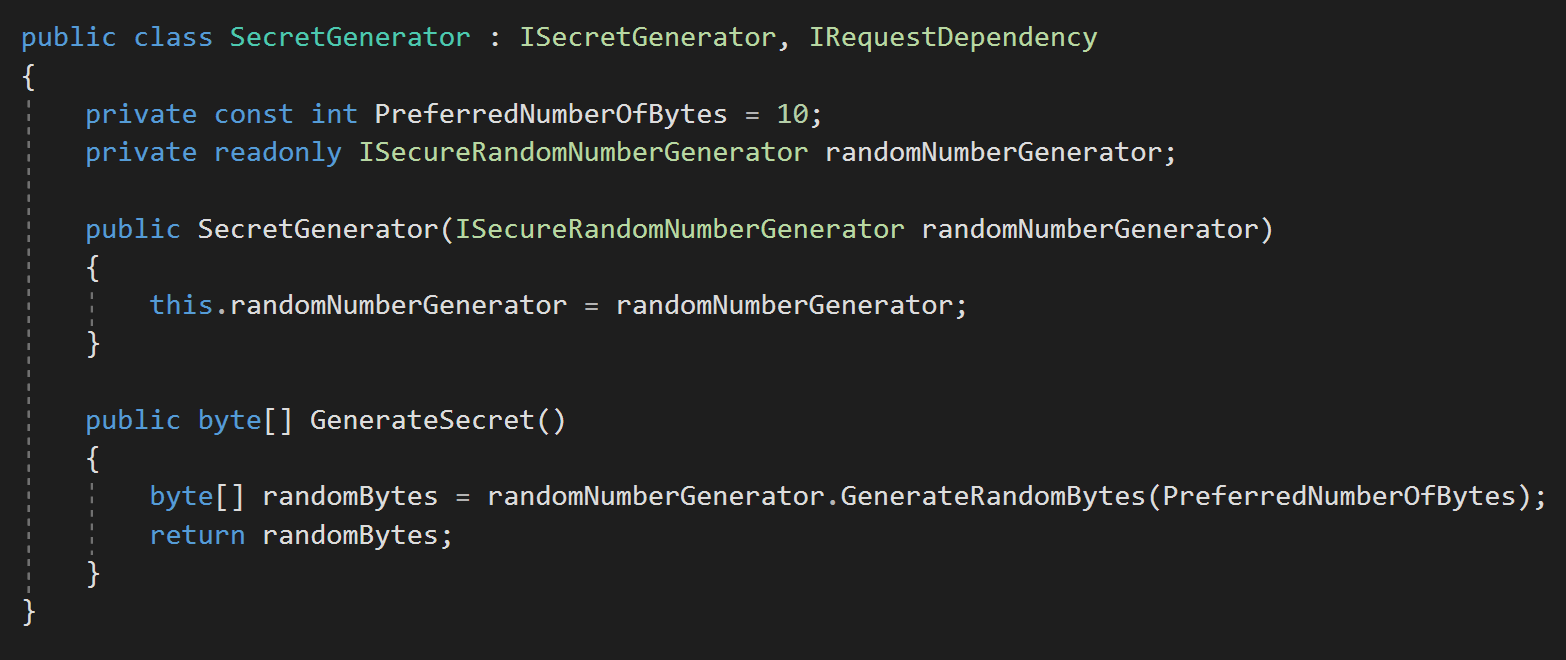
\includegraphics[width=\textwidth]{content/images/code-secretgenerator}
    \caption{Klasa generująca sekret użytkownika.}
    \label{code-secretgenerator}
\end{figure}
\begin{figure}[t]
    \centering
	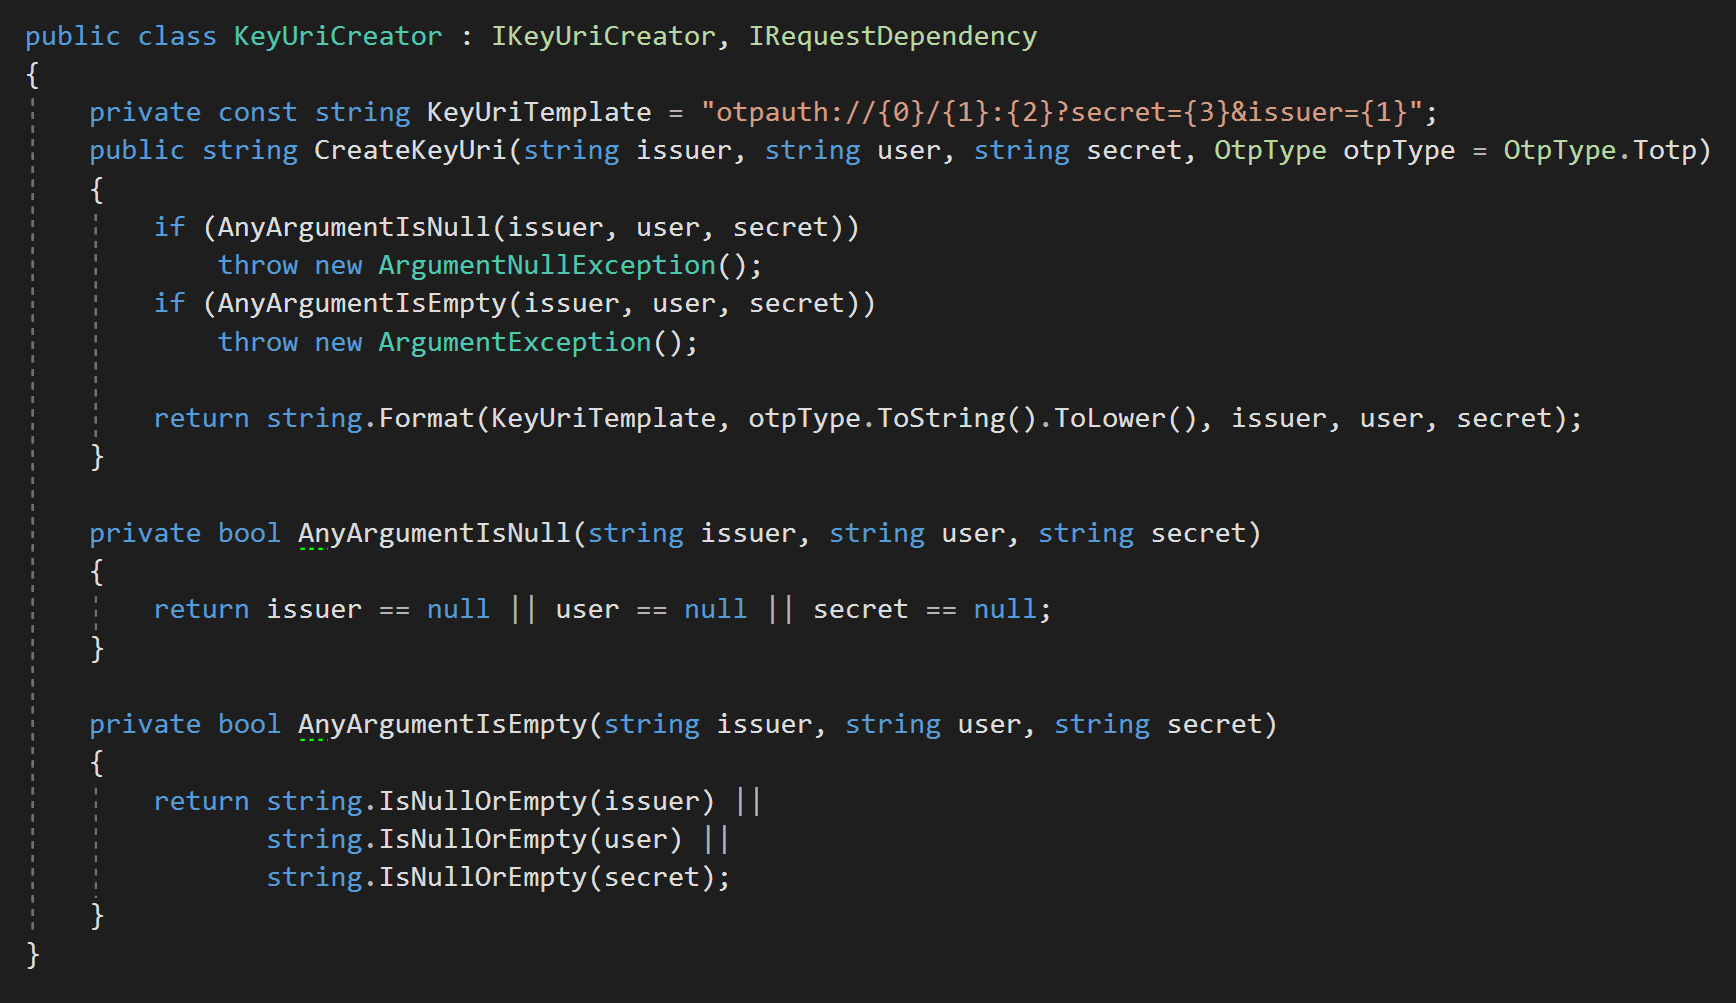
\includegraphics[width=\textwidth]{content/images/code-keyuri}
    \caption{Klasa generująca KeyUri.}
    \label{code-keyuri}
\end{figure}
\begin{figure}[t]
    \centering
	
\includegraphics[width=0.5\textwidth]{content/images/qr-hotp}
    \caption{Kod QR umożliwiający generację haseł typu HOTP.}
    \label{qr-hotp}
\end{figure}
\begin{figure}[t]
    \centering
	
\includegraphics[width=0.5\textwidth]{content/images/qr-totp}
	\caption{Kod QR umożliwiający generację haseł typu HOTP.}
    \label{qr-totp}
\end{figure}

\section{Generowanie OTP po stronie serwera}
\begin{figure}[t]
    \centering
	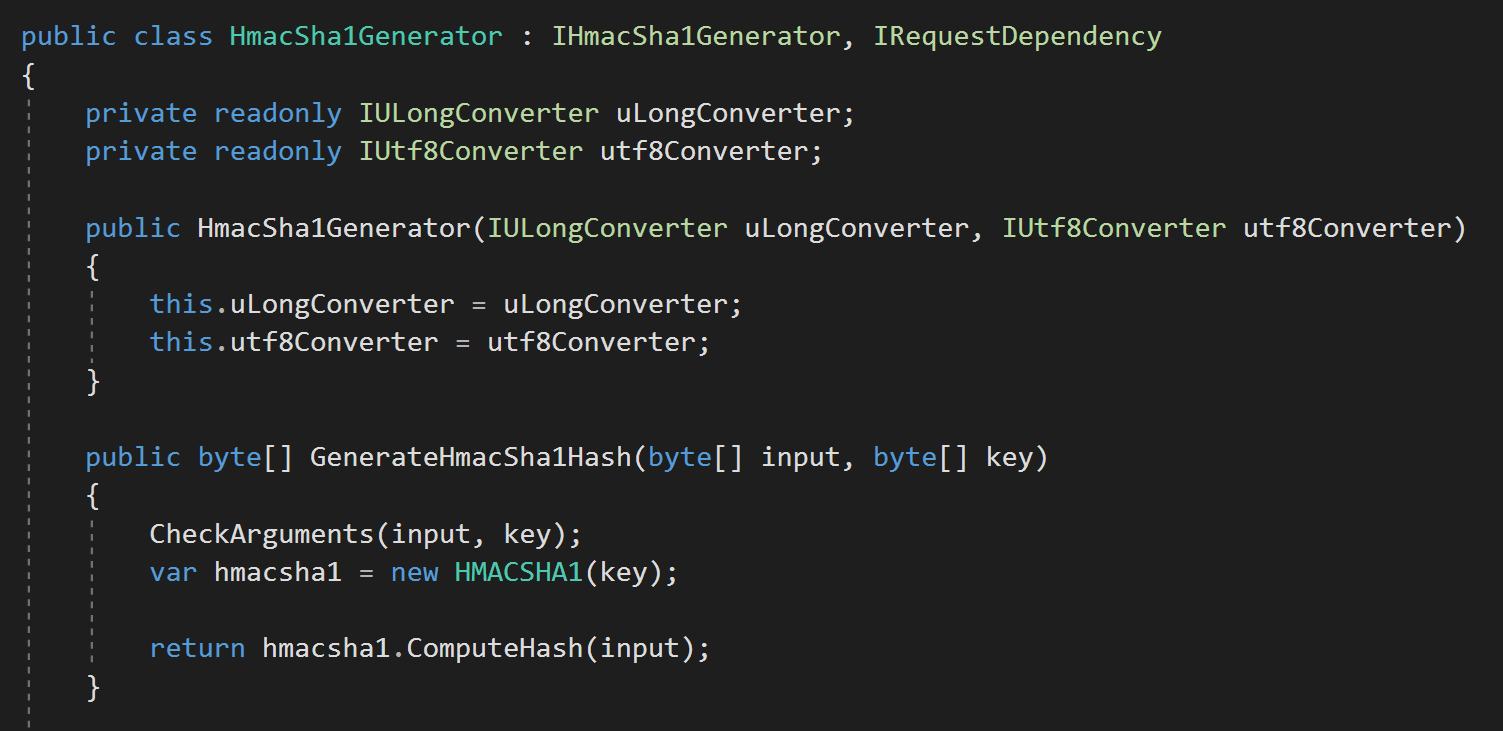
\includegraphics[width=\textwidth]{content/images/code-hmac}
    \caption{Klasa generująca HMAC.}
    \label{code-hmac}
\end{figure}
\begin{figure}[t]
    \centering
	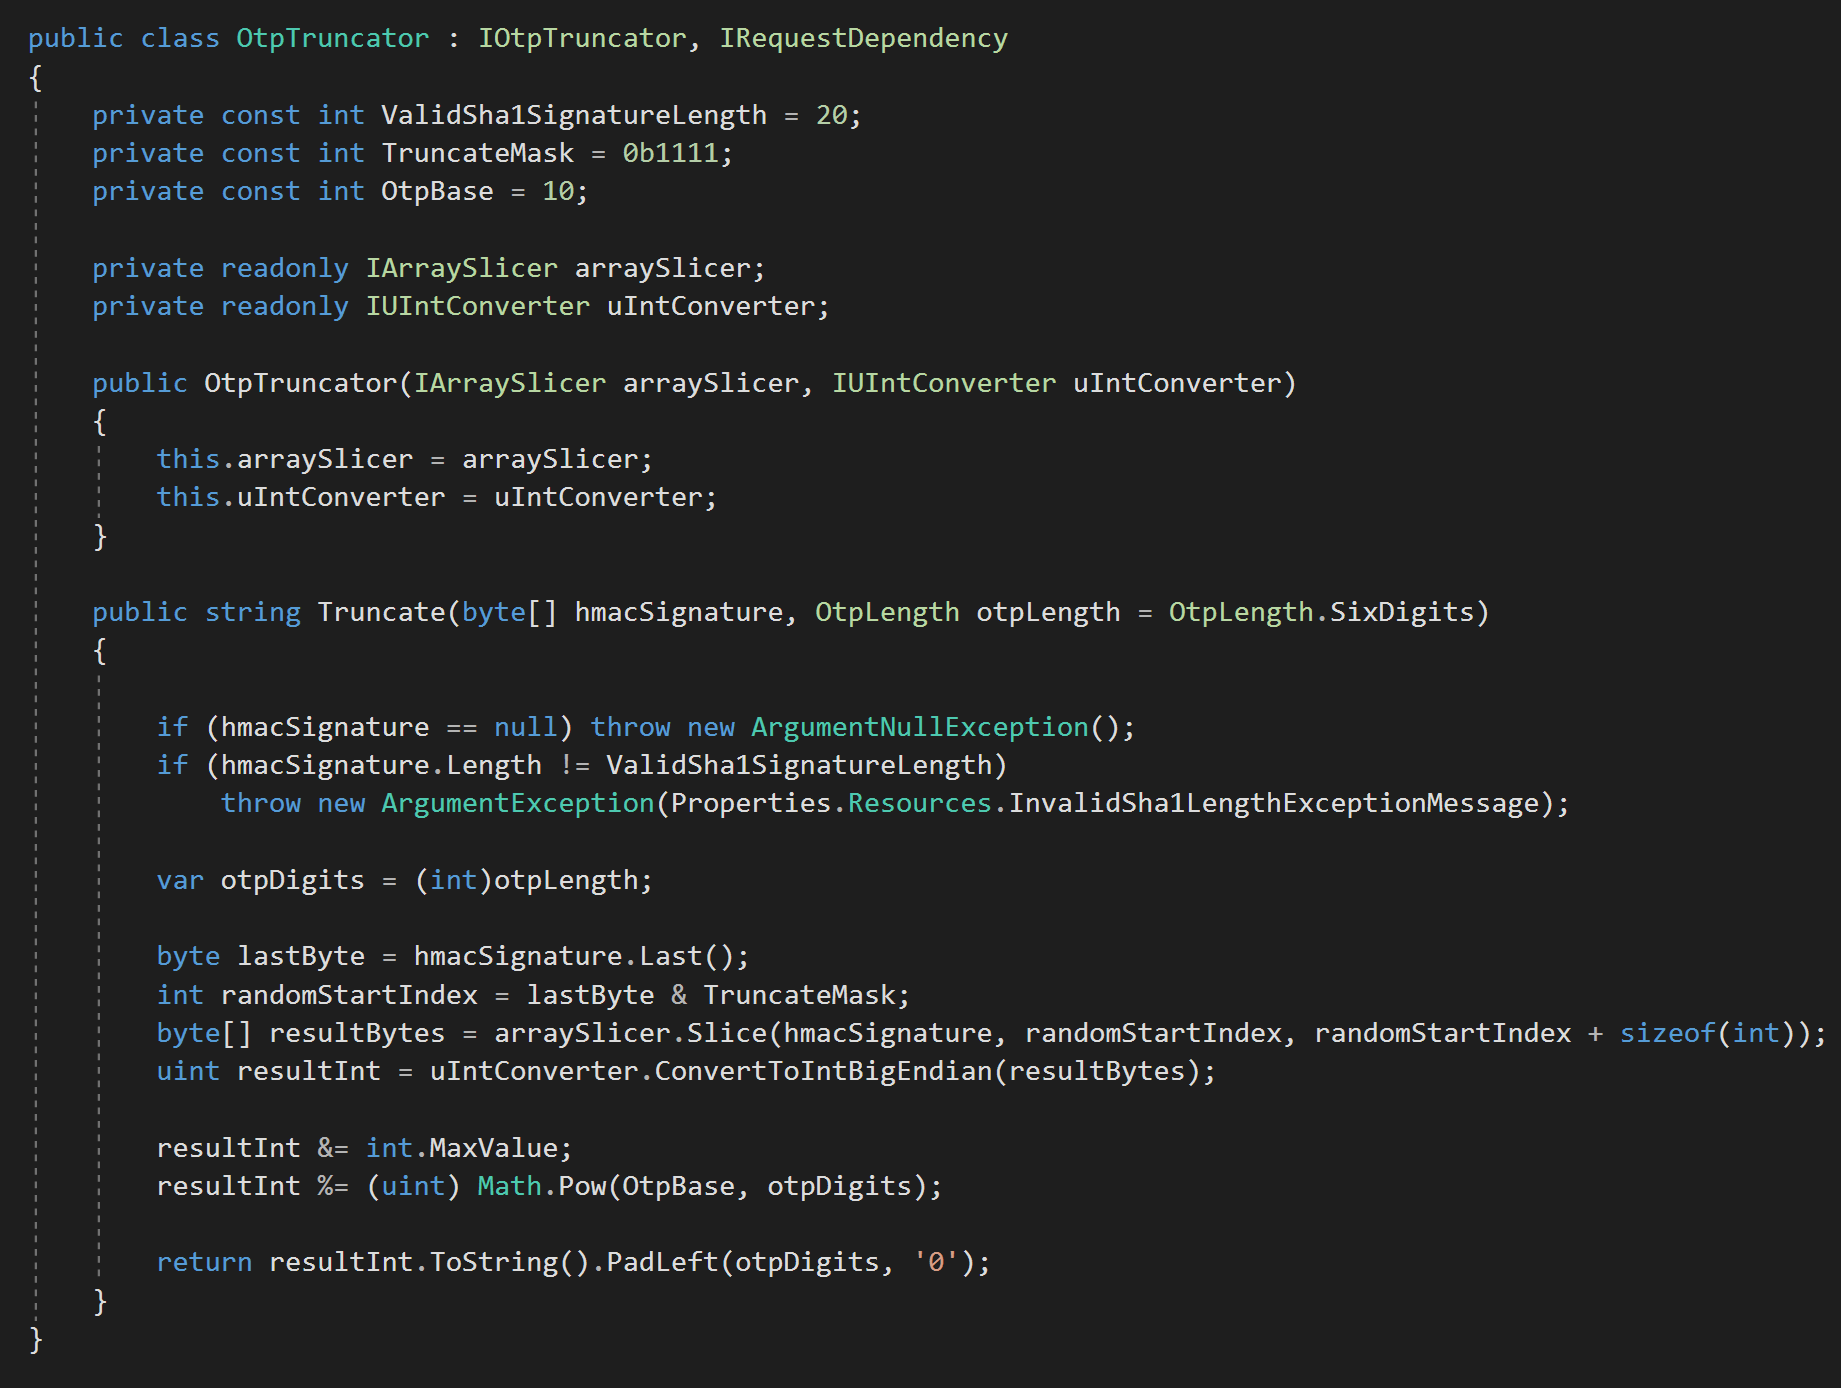
\includegraphics[width=\textwidth]{content/images/code-truncator}
    \caption{Klasa odpowiedzialna za przycięcie wyniku HMAC do postaci hasła.}
    \label{code-truncator}
\end{figure}
\begin{figure}[t]
    \centering
	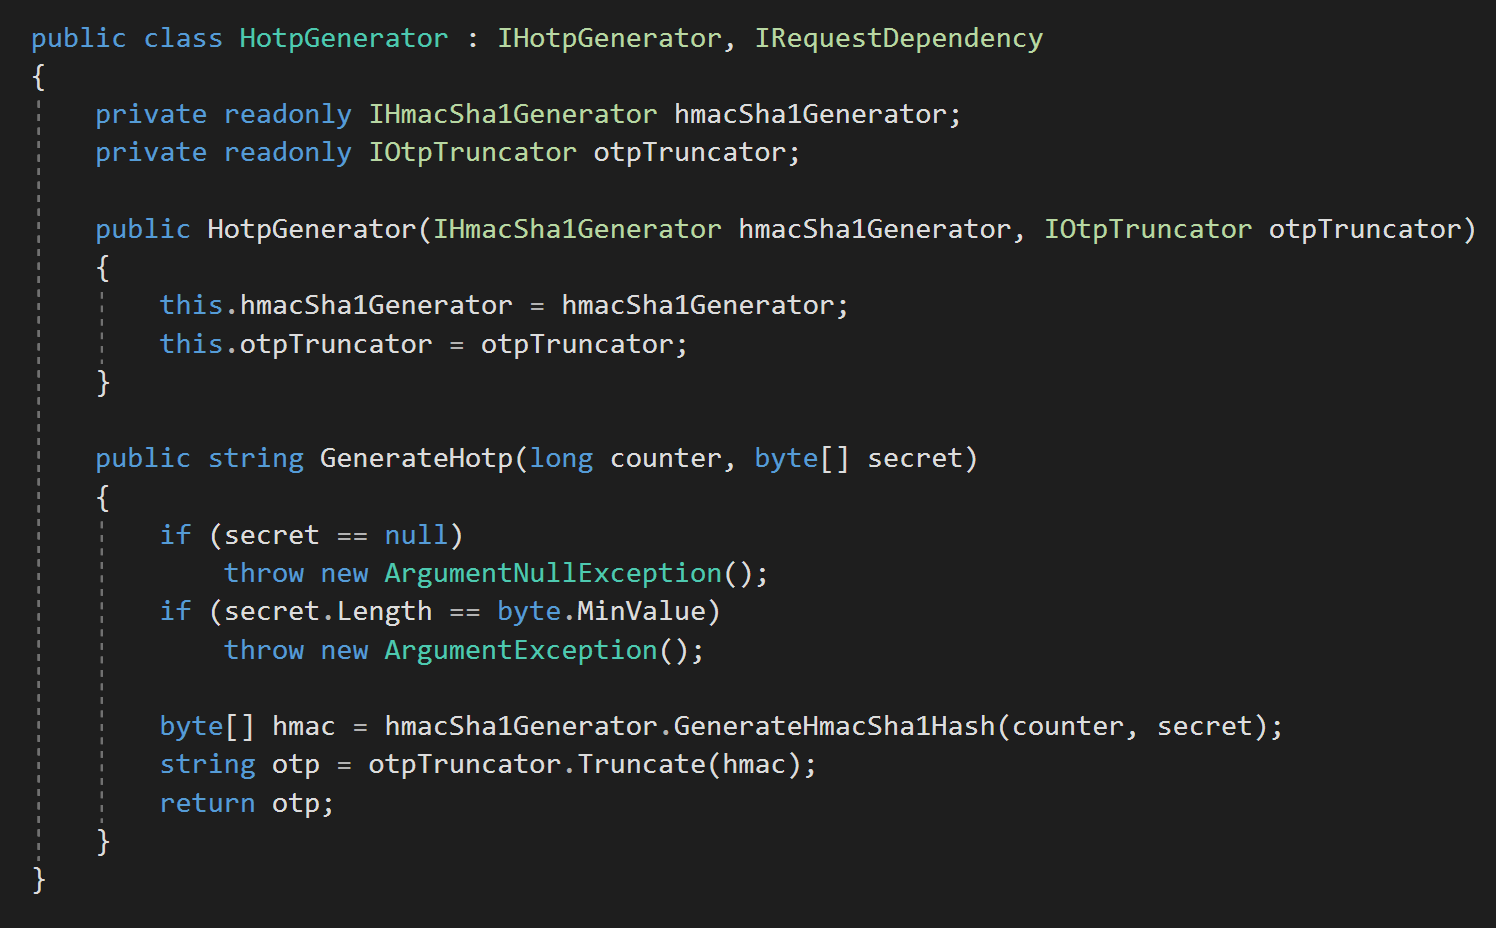
\includegraphics[width=\textwidth]{content/images/code-hotpgenerator}
    \caption{Klasa generująca hasło jednorazowe oparte o licznik.}
    \label{code-hotp}
\end{figure}
\begin{figure}[t]
    \centering
	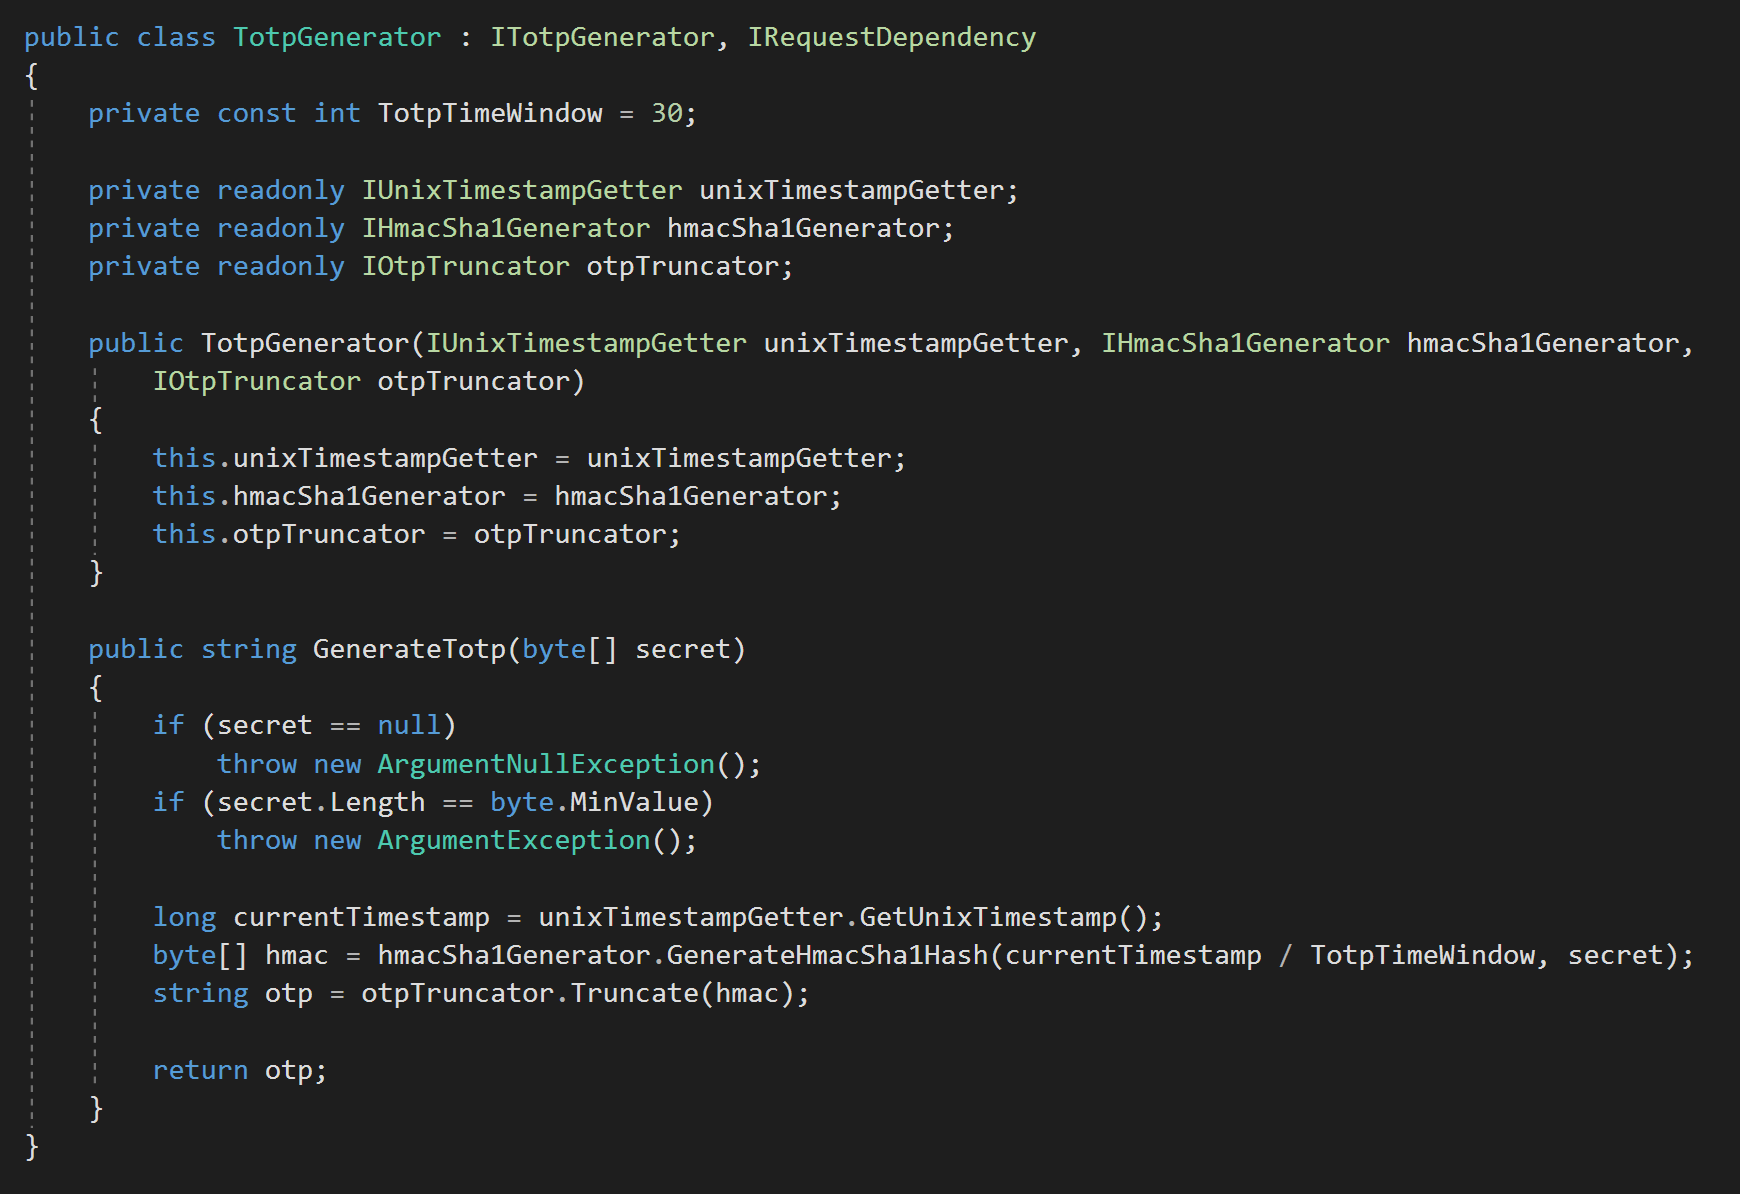
\includegraphics[width=\textwidth]{content/images/code-totpgenerator}
    \caption{Klasa generująca hasło jednorazowe oparte o czas.}
    \label{code-totp}
\end{figure}

\section{Generowanie OTP po stronie użytkownika}
\begin{figure}[t]
    \centering
	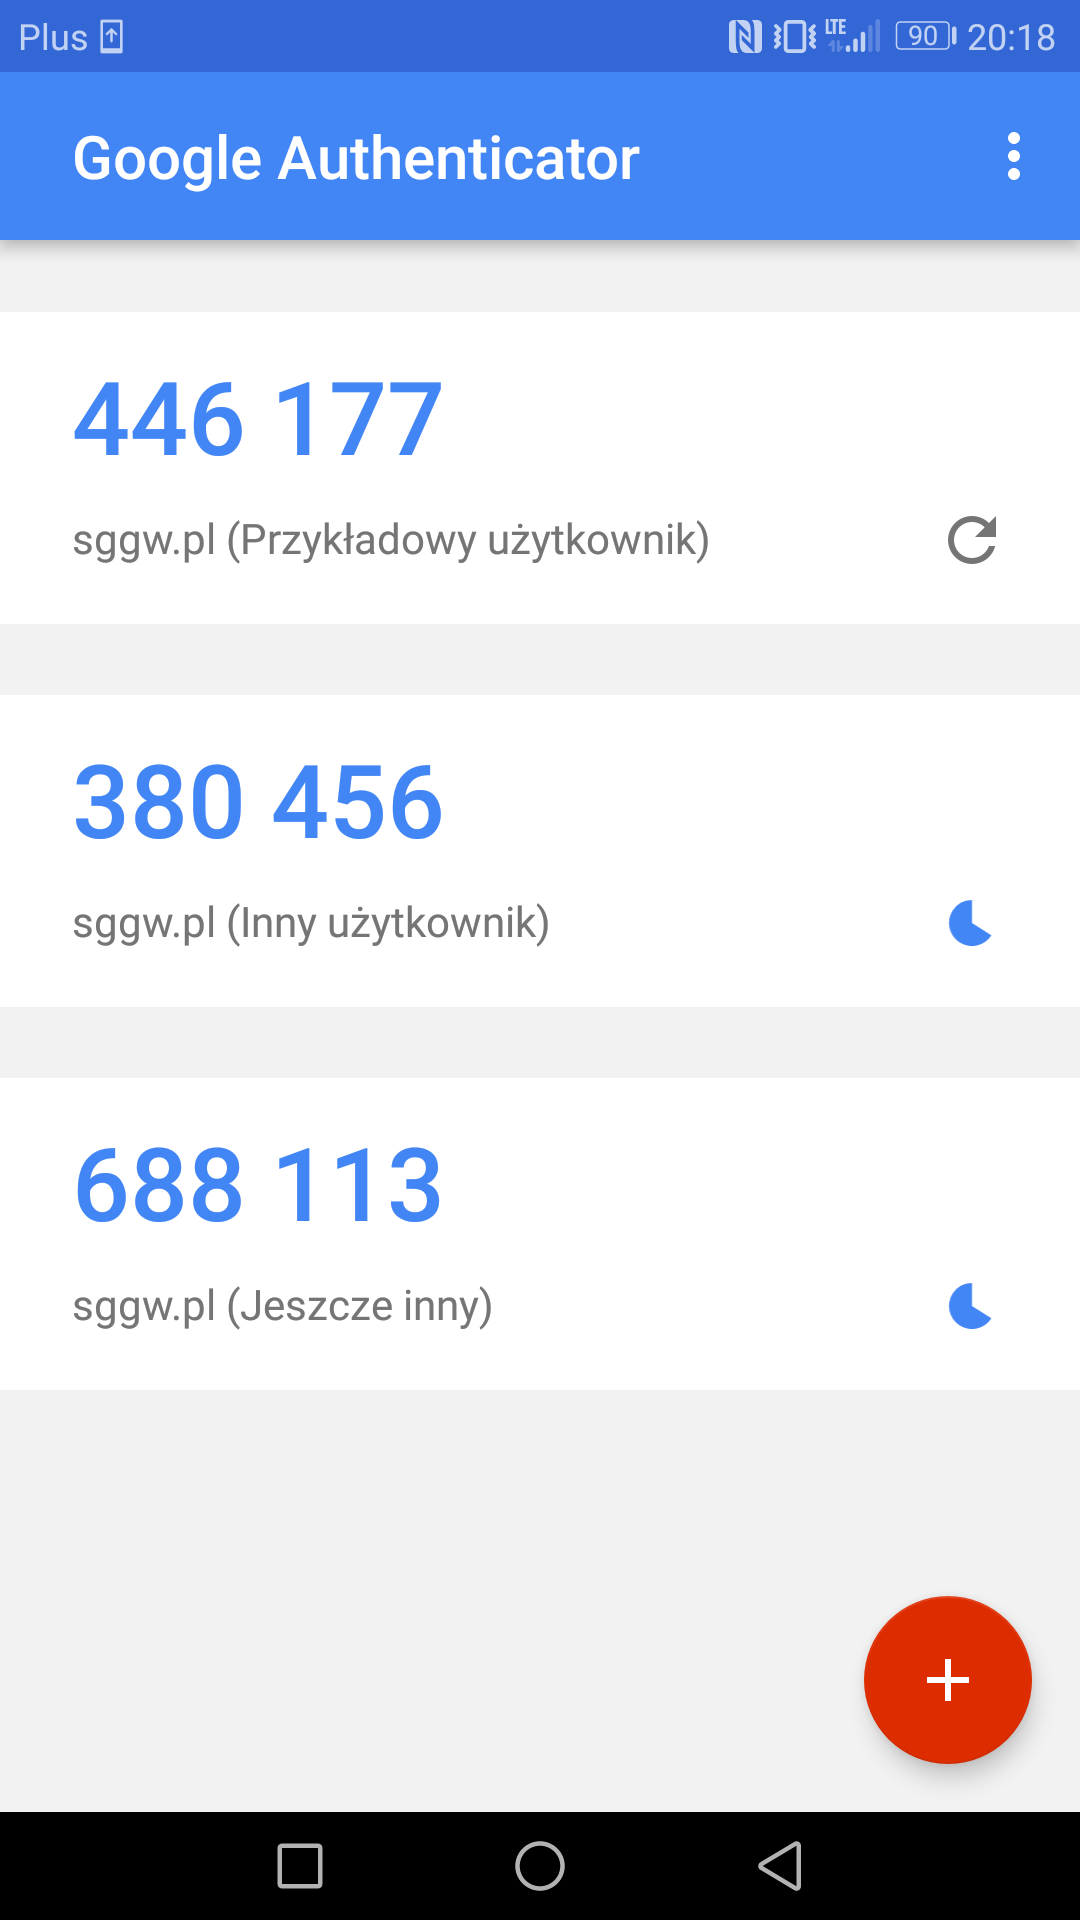
\includegraphics[width=0.5\textwidth]{content/images/mobile-google}
	\caption{Użycie aplikacji Google Authenticator.}
    \label{mobile-google}
\end{figure}
\begin{figure}[t]
    \centering
	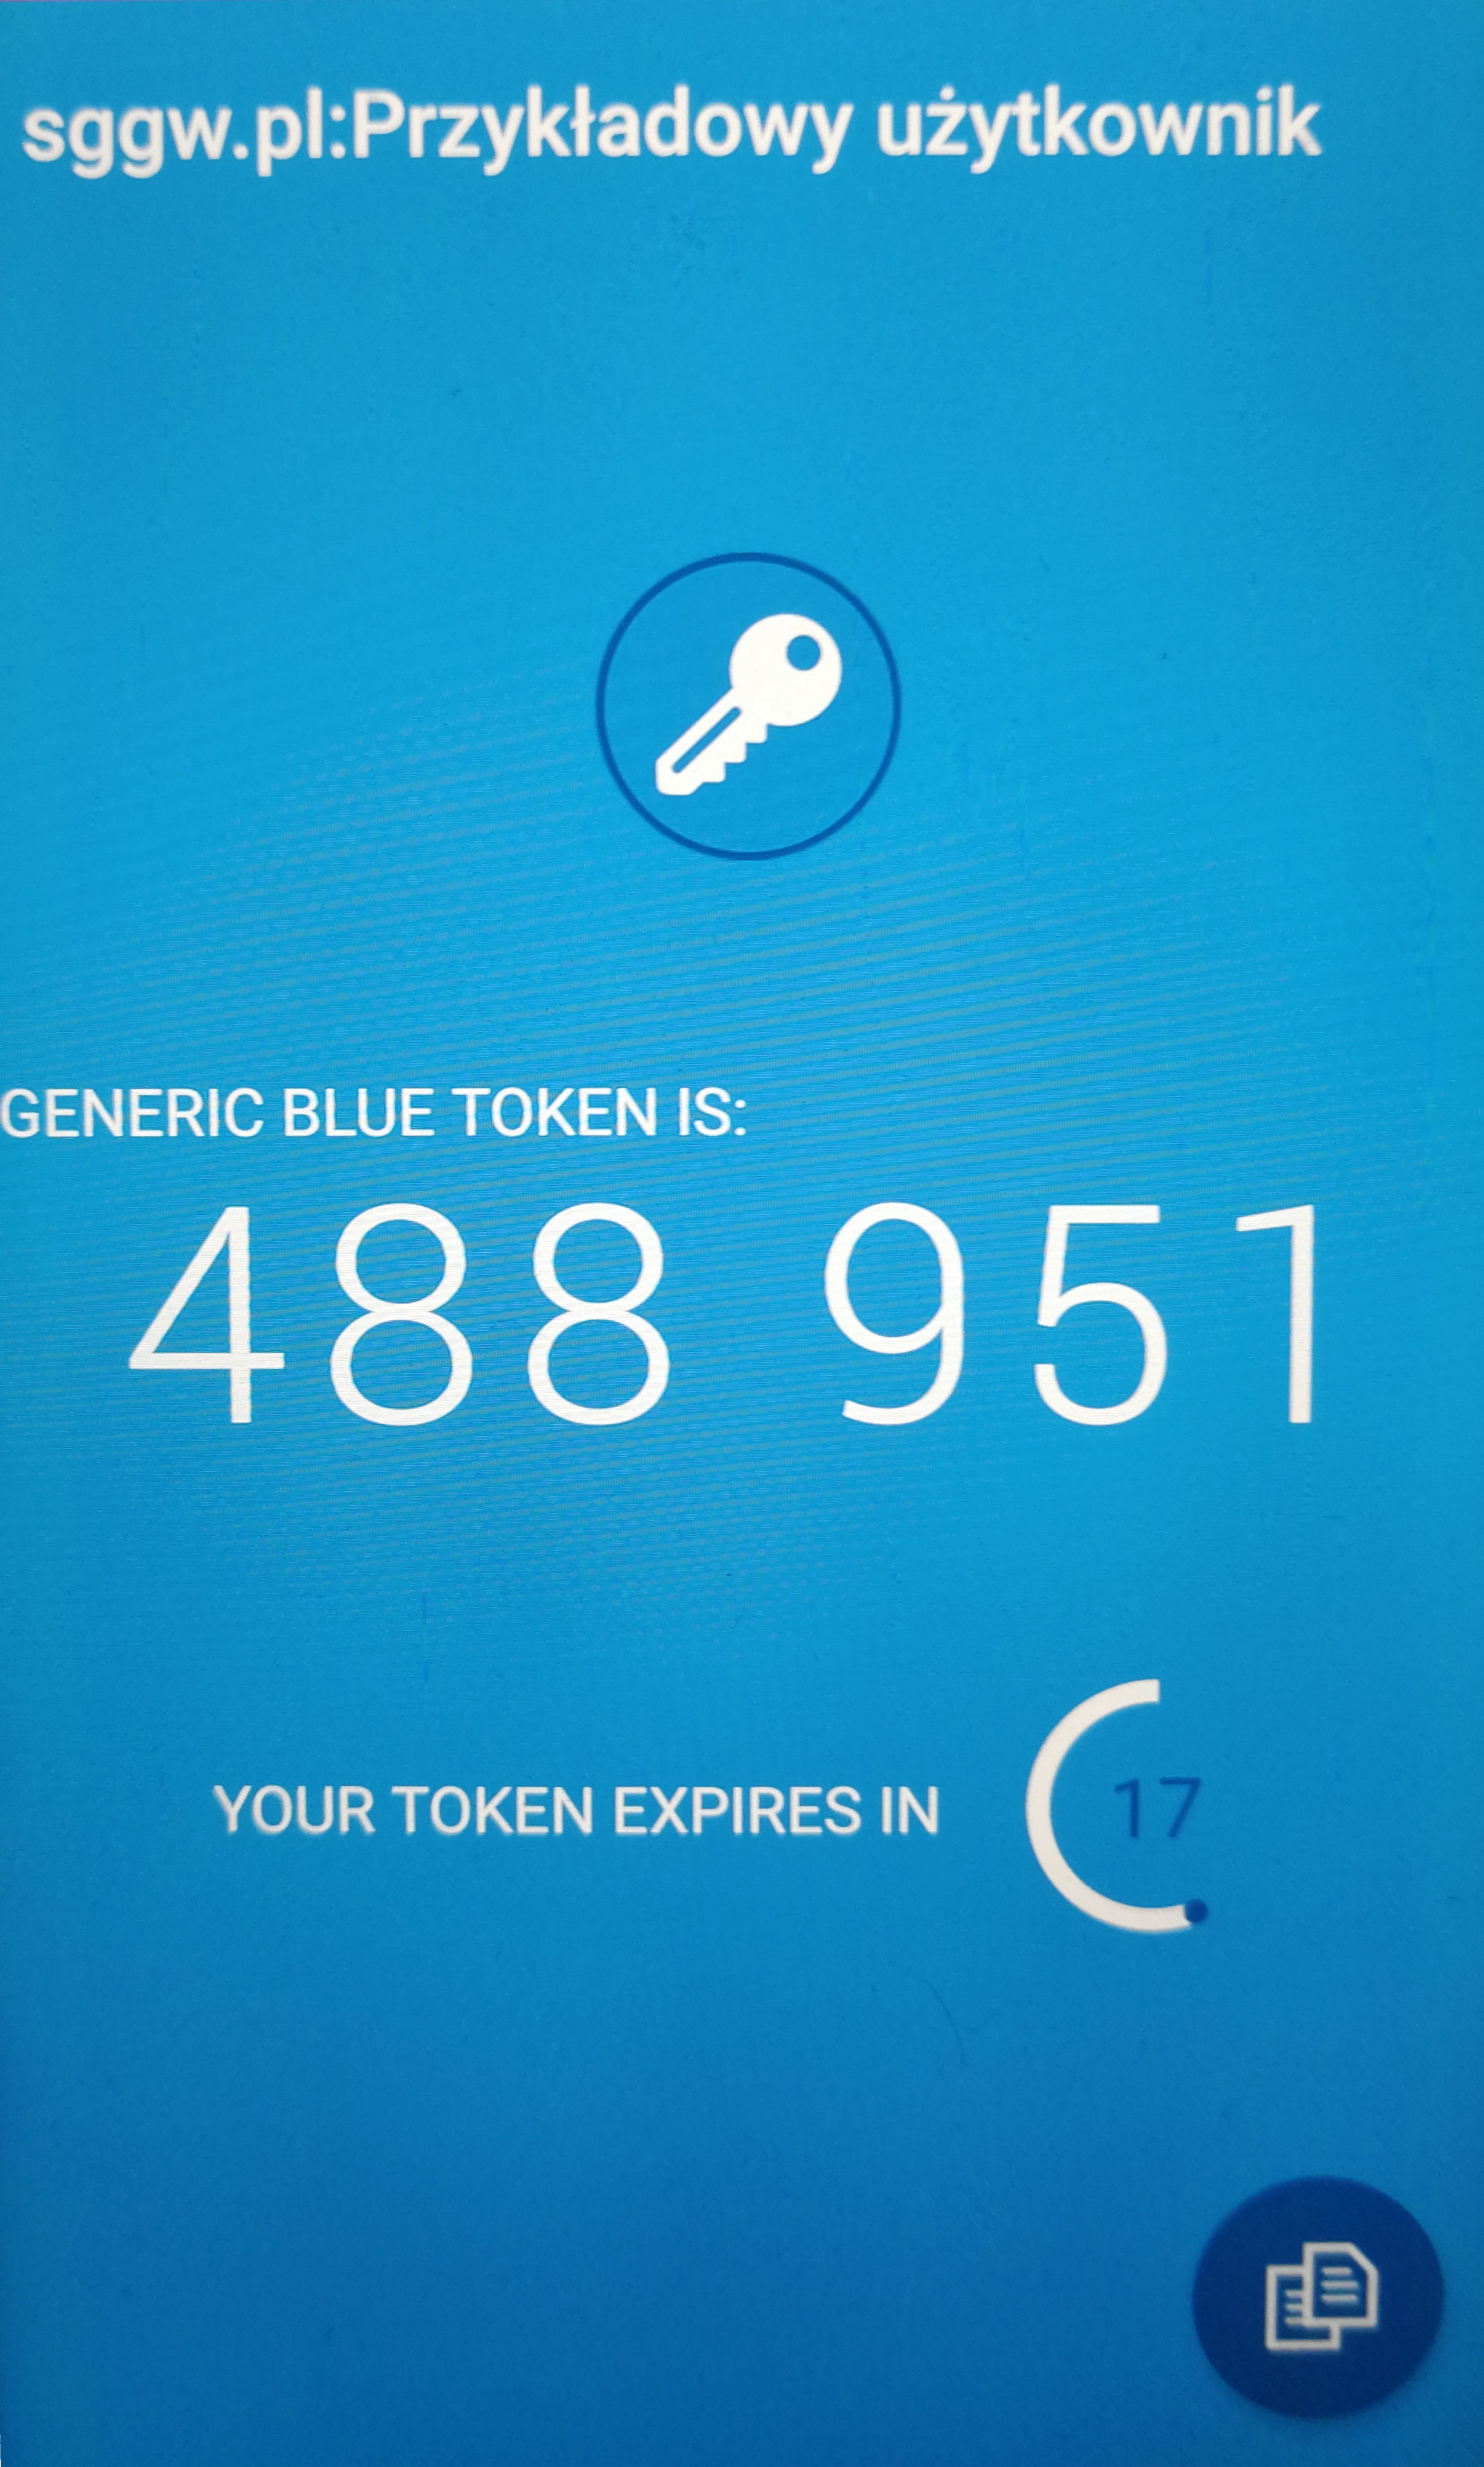
\includegraphics[width=0.5\textwidth]{content/images/mobile-authy}
	\caption{Użycie aplikacji Authy.}
    \label{mobile-authy}
\end{figure}

\section{Przechowywanie sekretu użytkownika}
\begin{figure}[t]
    \centering
	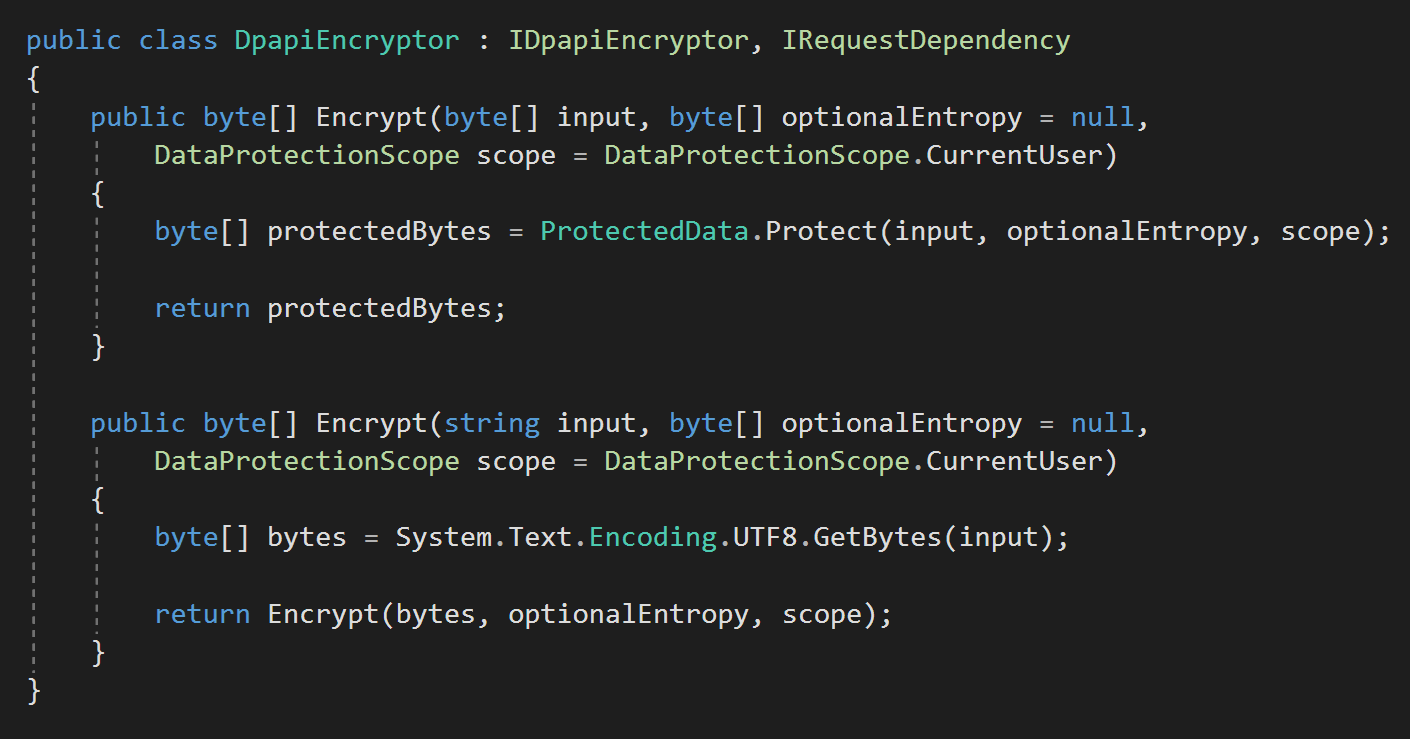
\includegraphics[width=\textwidth]{content/images/code-encrypt}
    \caption{Klasa odpowiedzialna za szyfrowanie.}
    \label{code-encrypt}
\end{figure}
\begin{figure}[t]
    \centering
	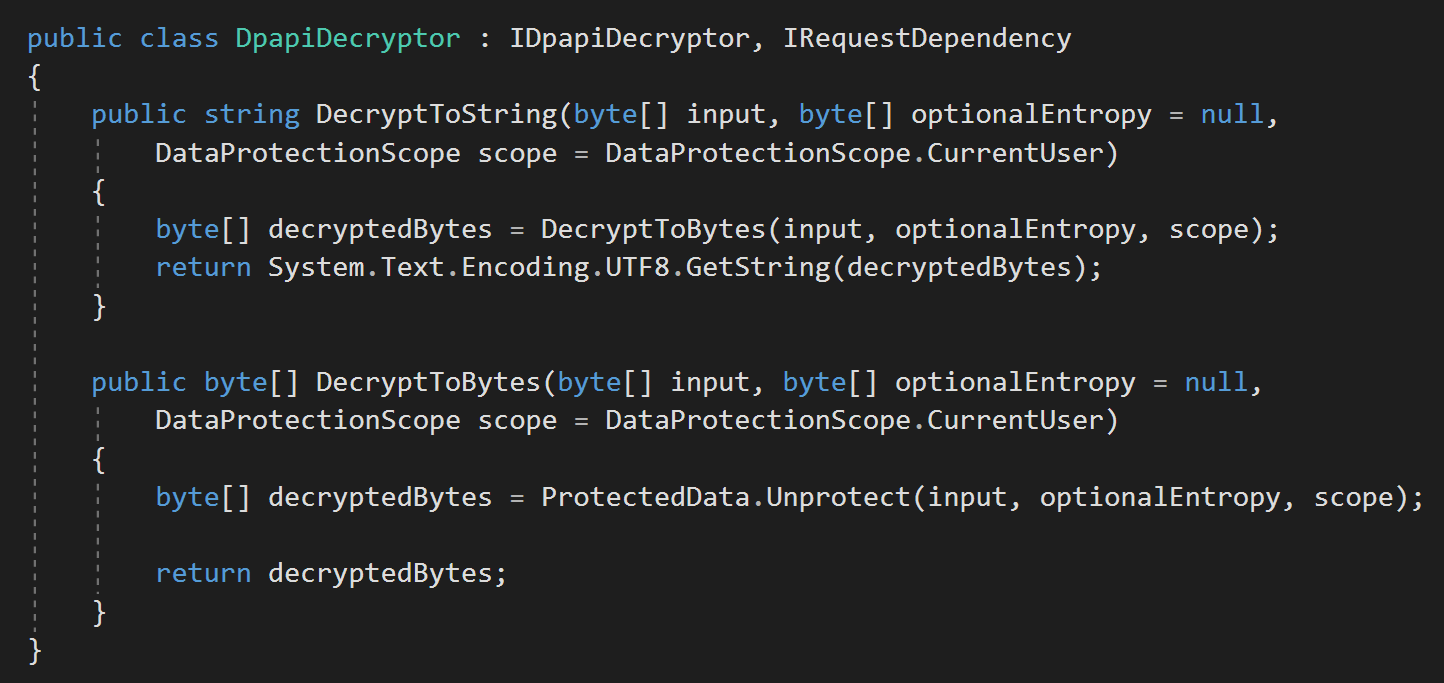
\includegraphics[width=\textwidth]{content/images/code-decrypt}
    \caption{Klasa odpowiedzialna za deszyfrowanie.}
    \label{code-decrypt}
\end{figure}
\section{Przykład użycia projektu}
\begin{figure}[t]
    \centering
	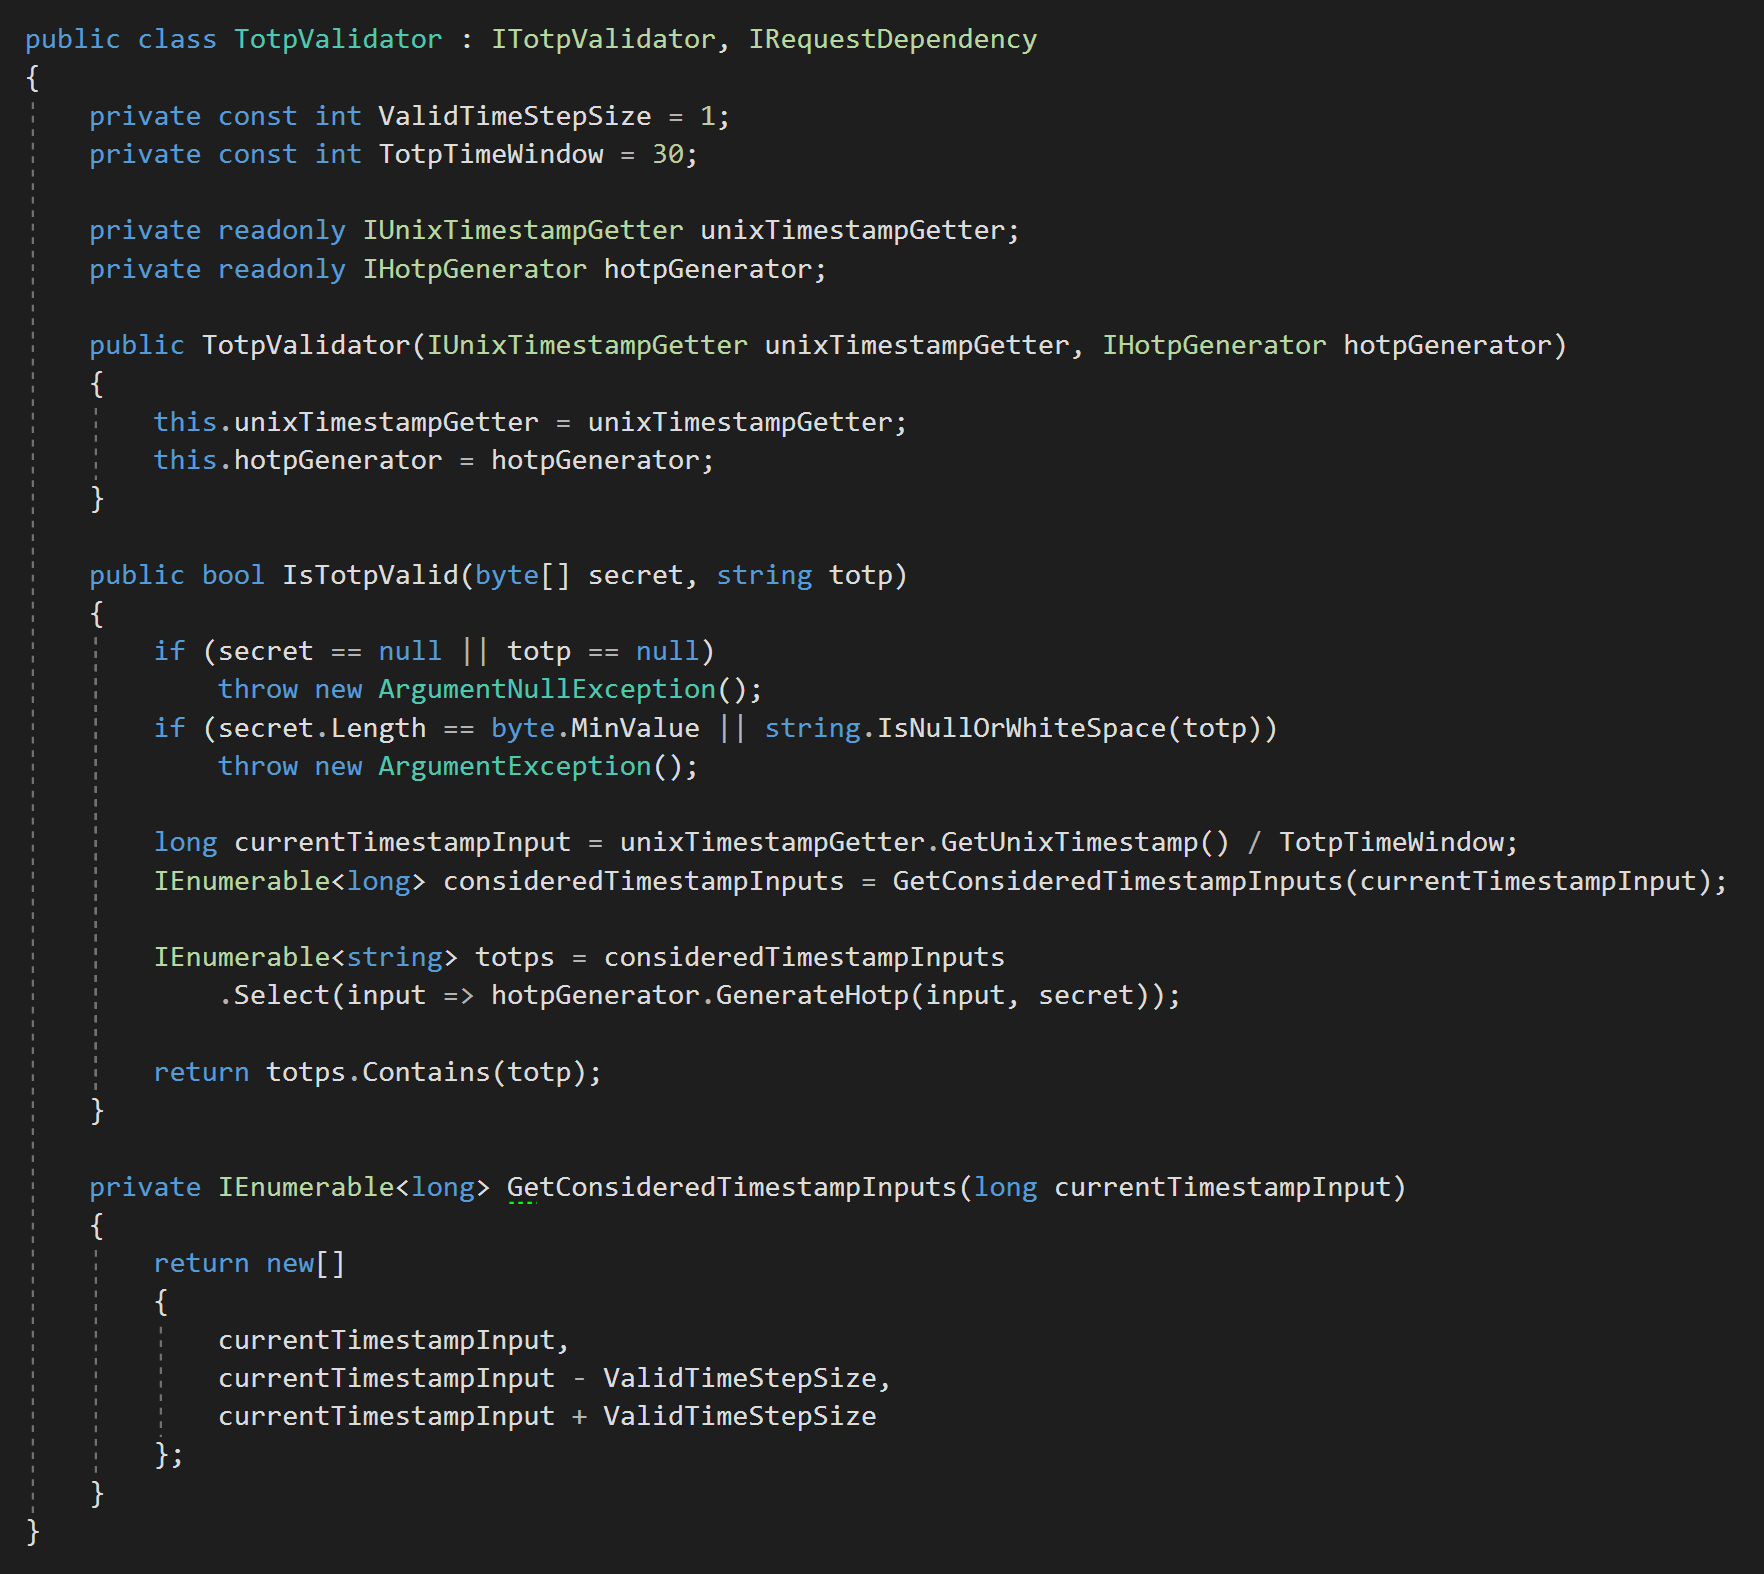
\includegraphics[width=\textwidth]{content/images/code-tvalidator}
    \caption{Klasa odpowiedzialna za walidację hasła typu TOTP.}
    \label{totp-validator}
\end{figure}

\section{Planowane ulepszenia}

\subsection{Generowanie hasła po stronie użytkownika}
Za najbezpieczniejsza metodę generacji haseł jednorazowych po stronie użytkownika uważany jest 
token sprzętowy, zabezpieczony kodem PIN. 
Jest to dosyć kosztowna metoda ze względu na koszty produkcji takiego tokenu, jak również 
jest mało uniwersalna, gdyż zwykle token powiązany jest z pojedynczym kontem. \\
Wychodząc na przeciw tym ograniczeniom, mogą tutaj zostać zaproponowane rozwiązania 
oparte o mikrokontroler \textit{Arduino Uno} lub o mini-komputer \textit{Raspberry Pi Zero}.
Projekt ten mógłby mieć formę DIY (Do it yourself) czyli być przepisem jak z dostarczonego 
oprogramowania i części stworzyć własny token sprzętowy, mogący generować hasła jednorazowe do wielu serwisów. 
Token posiadałby ekran, na którym wyświetlane by było wygenerowane hasło jedno razowe oraz klawiaturę 
alfanumeryczną, wykorzystywaną do podawania kodu PIN oraz do dodania nowego konta do bazy tokenu.

\subsection{Biblioteki klienckie}
Użycie REST API jest możliwe w każdej technologii umożliwiającej wykorzystanie protokołu HTTP 
wraz z formatem JSON. 
Dużo wygodniejsze jest jednak korzystanie z gotowych bibliotek, stworzonych pod daną technologię. \\ \\
W tym celu, w kolejnych wersjach projektu, planowana jest implementacja bibliotek klienckich w następujących 
językach programowania:
\begin{itemize}
	\item{C}
	\item{C++}
	\item{Clojure}
	\item{D}
	\item{Elixir}
	\item{Erlang}
	\item{Groovy}
	\item{Java}
	\item{JavaScript}
	\item{Kotlin}
	\item{Nim}
	\item{Objective-C}
	\item{Perl}
	\item{PHP}
	\item{Scala}
	\item{Swift}
\end{itemize}

\subsection{Architektura}
Możliwe jest także ulepszenie architektury części REST API projektu pod kątem większego odseparowania od siebie komponentów.
Szczególnie dotyczy to odseparowania części przechowującej sekrety użytkowników i walidującej hasła jednorazowe od reszty
aplikacji. 
W~idealnym przypadku odseparowana część umieszczona by była na osobnym systemie komputerowym, bez dostępu do Internetu. 
Komunikacja z główną częścią aplikacji powinna odbywać się wtedy poprzez minimalny interfejs, pozwalający wyłącznie na 
uwierzytelnienie podmiotu oraz walidację podanego przez użytkownika hasła jednorazowego. 
Po przesłaniu podanego przez użytkownika hasła jednorazowego, 
zwrócony zostałby jedynie wynik walidacji w postaci \textit{true} lub \textit{false}.

\subsection{Konteneryzacja części serwerowej}
Poza podstawowym przypadkiem użycia opartym o REST API wystawione pod adresem \texttt{https://picnicauth.gear.host/swagger/ui/index},
nic nie stoi na przeszkodzie wykorzystaniu kodu źródłowego aplikacji i stworzenia REST API na własnym serwerze, na przykład w firmowej
sieci lokalnej. Ten sposób wykorzystania projektu może okazać się bardziej bezpieczny, jeśli jest przez dany podmiot 
umiejętnie administrowany oraz zupełnie niebezpieczny w przeciwnym przypadku. \\
Aby ułatwić procedurę wdrożenia REST API na serwer można zaproponować tutaj użycie kontenerów. 
Dzięki nim aplikacja nie jest zależna od systemu, który jest zainstalowany na serwerze a sam proces wdrożenia jej
jest niezwykle prosty i szybki.
Może zostać użyte oprogramowanie \textit{Docker}. 

\subsection{Przechowywanie sekretu}
Obecnie do szyfrowania sekretów użytkowników wykorzystywany jest interfejs \textit{Windows Data Protection}. 
Posiada on kilka wad, między innymi to, że jest silnie zależny od hasła użytkownika sytemu. 
Lepszym ale i bardziej kosztownym rozwiązaniem, byłoby użycie szyfrowania sprzętowego zamiast wspomnianego interfejsu.
